\subsection{Safety Constraint}
\label{text:approach/constraint/safety}
As pointed out in Chapter \ref{text:introduction} one of the main advantages of an optimization-based approach for robot navigation in human crowds is the possibility to ensure safety, namely by posing safety guarantees in form of constraints to the optimization problem. Infusing safety into a dynamical and probability system is not trivial, and widely dominated by approaches using chance-constraints. 

\subsubsection{Chance Constraints}
Sampling-based methods relying on the Bernstein approximation \cite{Calafiore2005}, on scenario planning approach \cite{Bemporad1999} or on Monte Carlo sampling \cite{Hong2011}\cite{Janson2015} as well as dynamic-programming based approaches for discrete space \cite{Yin-LamChow2013}\cite{Ono2015} \cite{Chow2015a} have been purposed. While these methods work for general distributions but usually lack are too slow for an online optimization approach, shrinking the space of distributions can improve the performance, such as in \cite{Chen2018}\cite{Calafiore2006}\cite{Carvalho2014}\cite{Blackmore2009}\cite{Blackmore2011}. 
\newline
However as stated in \cite{Lew2020} these approaches are slow for a large number of obstacles. In the context of \project the pedestrians ("obstacles") are assigned to multi-modal distributions. While the most of the previously mentioned work on sampling-free chance constraints focus on uniformly radial distributions, e.g. Gaussians, none of them takes multi-modality into account. To do so, a chance constraint could be formulated individually for each mode of a multi-modal distribution, and weighed by multiplying the mode's importance weight $\pi_m$, might be a feasible approach. For each pedestrian $k$, mode $m$, prediction time-step $t$ and probability threshold $p$ the chance-constraint would then be:

\begin{equation}
\piped[k,m]_t \cdot Pr(g_t^{k,m}(x)\leq 0) \geq p
\end{equation}

However, doing so entails repeatedly calling the prediction model $\distmodel[]$. Constraining the sum or product of the mode-wise chance constraints instead, by using Boole's inequality, would be very conservative. In any way using chance-constraints the evaluation of the set of resulting constraints would be at least linear with the number of pedestrians, the number of modes and the length of the planning horizon. While the constraint evaluation can be batched, programmatically each constraint has to be differentiated individually (as required by the PyTorch automatic differentiation engine \cite{pytorch}), which is the main bottleneck of the whole trajectory optimization problem. 

\subsubsection{Hamilton-Jacobi Reachability} 
Reachability analysis deals with the problem of a two-person, zero-sum differential game, specifically it tries to solve the question how to react if there is another player that interferes with the fulfillment of the robot's objective by optimizing the joint system state, assuming that the counter-player always counters the robot's action optimally, i.e. assuming the worst case disturbance $\d = \beta[\u]$ \cite{Pavone2020}. Under these conditions the optimal control strategy can be derived by maximizing: \\

\begin{equation}
V(x(t), t) = \min_{\beta[\u](\cdot)} \max_{\u(\cdot)} \left[ \int_t^0 l(\x(\tau), \u(\tau), \boldsymbol{d}(\tau)) \, d\tau + l_f(\x(0)) \right]
\label{eq:j_reachability}
\end{equation}

with $(\x(\tau), \u(\tau), \d(\tau))$ describing the joint system with dynamics $f(\boldsymbol{x}, \u, \d)$. While solving for the robot's optimal control strategy $\u_{opt}$ in open-loop (also \textit{forward} reachability) is computationally cheap, but leads to overly conservative and hence un-realistic estimates, since the counter-player knows the entire policy $\u_{opt}$ in advance and can re-act regardingly, \ac{HJR} (also \textit{backward} reachability) addresses the problem of maximizing Equation \ref{eq:j_reachability} in closed-loop, i.e. by allowing the robot to adapt its control policy at each time-step. As proven in \cite{Pavone2020} this is equivalent as solving the Hamilton-Jacobi-Isaacs differential equation with boundary condition: \\

\begin{problem}{General \ac{HJR} problem}
\begin{align}
\pd{V}{t} + \max_{\u}  \min_{\d} &\left[l(\x, \u, \d) + \nabla V^T f(\x, \u, \d) \right] = 0 \\ 
V(\x, 0) &= l_f(\x) \\
\Rightarrow \u_{opt} &= \arg \max_{\u}  \min_{\d} \nabla V^T f(\x, \u, \d)
\label{eq:hjr_problem_u}
\end{align}
\label{eq:hjr_problem}
\end{problem}

Solving Problem \ref{eq:hjr_problem} has been examined for several scenarios and applications over the recent years, as in \cite{Dhinakaran2017}\cite{Margellos2009}\cite{Chen2017b}. In opposite to forward reachability \ac{HJR} finds the non-overly conservative avoidance maneuvers, "stemming from its equivalence to an exhaustive search over the joint system dynamics", while still being flexible with respect to the system dynamics, as depicted by \cite{Leung2020}. To solve \ref{eq:hjr_problem} the value function $V(\cdot)$, as well as its gradient, are computed for every cell of a $n$-dimensional grid that discretizes the joint state $\x(\tau)$ and for some discrete time horizon (including $\tau \rightarrow \infty$). 

\paragraph{\ac{HJR} in single pedestrian scenario}
In case of a single pedestrian, Problem \ref{eq:hjr_problem} can be understood as a "run-and-catch" game, in which the pedestrian, the "disturbance", takes actions to decrease the distance between robot and pedestrian while the robot counter acts on that. Therefore a circular avoid set $\xset_{avoid}$ is defined around the pedestrian with radius $R_{avoid} = 1m$. Then the value function can be interpreted as the set of joint states from which a collision between robot and pedestrian might occur after time $T_{HJR}$.
\newline
Figure \ref{img:hj_game} displays the avoid set around the pedestrian in a static case, i.e. when only the robot would move. Then, Problem \ref{eq:hjr_problem} breaks down to determining a value for each robot control policy, which is larger then zero for un-rolled trajectories that do not touch $\xset_{avoid}$ (safe), while being larger smaller than zero otherwise (unsafe).

\begin{figure}[!ht]
\begin{center}
\begin{tikzpicture}

    \node[inner sep=0pt] (ped) at (5,1)
    {
\includegraphics[width=.05\textwidth]{images/walking.png}};
    \node[inner sep=0pt] (robot) at (-3,0)
    {
\includegraphics[width=.05\textwidth]{images/robot.png}};
       
    \fill[orange, opacity=0.3] (ped) circle (2);
    \node[] (D) at (5, 2){$\xset_{avoid}$};
    
    \draw [thick, dashed] (robot) to[out=0, in=180] (5,-0.5) to[out=0, in=180] node[above, sloped] {$\Vrel < 0$} (10, 1);
    
    \draw [thick] (robot) to[out=0, in=180] (5,3) to[out=0, in=180] node[above, sloped] {$\Vrel \geq 0$} (10, 1);  
    
\end{tikzpicture}
\end{center}
\caption{Avoid set for static ($\dxped[]_t = 0$), single pedestrian scenario}
\label{img:hj_game}
\end{figure}

The coupled system state describes the direction-wise distance between robot and pedestrian $\x - \xped[]$ as well as the robot's velocity $\dx$. As previously pointed out the pedestrian is modeled as a single integrator, so that its velocity $\dxped[]$ is a control input rather than a state variable. With the disturbance being the pedestrian's velocity $\dxped[] = \d$, the coupled system dynamics $\frel$ are: 

\begin{equation}
\frel(\x, \xped[]) = 
\begin{bmatrix} 
\dot{x} - \dot{\tilde{x}} \\  
\dot{y} - \dot{\tilde{y}} \\  
\ddot{x} \\
\ddot{y} 
\end{bmatrix} = 
\begin{bmatrix} 
\dx - \dxped[] \\ 
\u
\end{bmatrix}
\label{eq:hj_dynamics}
\end{equation}

By solving Equation \ref{eq:hjr_problem_u} for the given coupled system dynamics, the robot's optimal control action $\u_{opt}^{HJR}$, regarding Problem \ref{eq:hjr_problem}, is determined as by maximizing:

\begin{equation}
\arg \max_{\u} \nabla \Vrel \cdot \frel(\x, \xped[]) = \arg \max_{\u} (d\Vrel u_x + d\Vrel u_y) = 
\begin{cases}
u_{max} & \text{if } d\Vrel \geq 0 \\
u_{min} & \text{if } d\Vrel < 0	
\end{cases}
\label{eq:hj_u_opt}
\end{equation}

Similarly the worst-case disturbance can be derived as being the disturbance extremum which is opposite to the sign of the value function's gradient. For this specific  dynamics function the min- and max-operator are exchangeable in order (minimax-theorem), so that the optimal disturbance and control can be regarded independently.
\newline
Figure \ref{img:hj_value_function} displays two-dimensional slices of the four-dimensional value function. Thereby the left plot shows the one-dimensional case, i.e. $y = 0$ and $v_y = 0$. In particular, it is worth to mention that the value function is mostly linear. Note that the asymmetry with respect to $x = 0$ originates from the differences in maximal and minimal speed between robot and pedestrian, respectively.  In fact the pedestrian is assumed to have a larger maximum speed compared to the robot, as further discussed in Chapter \ref{text:experiments}. As a consequence value function's gradient is strictly non-positive for a time-horizon $T_{HJR} > 0$, meaning no matter no matter what the robot does the value function will not increase over time, since the pedestrian can always choose an action that decreases the distance between both agents:

\begin{equation}
\nabla \Vrel < 0 \quad \forall \xrel \in \xset_{rel} \smallsetminus \{ \boldsymbol{0} \}
\label{eq:hj_value_negative}
\end{equation}

Besides, the value function is symmetric in direction $x$ and $y$, as demonstrated in the right plot of Figure \ref{img:hj_value_function}, which can easily be derived from Equations \ref{eq:hj_dynamics} and \ref{eq:hj_u_opt}. The value function and its gradient has been computed using the \textit{helperOC} Matlab toolbox \cite{Bansal2017}, which harnesses level set methods.\footnote{For more information please visit my toolbox's fork on GitHub \href{https://github.com/simon-schaefer/HJReachibility}{HJReachability Toolbox}}

\begin{figure}[!ht]
\begin{center}
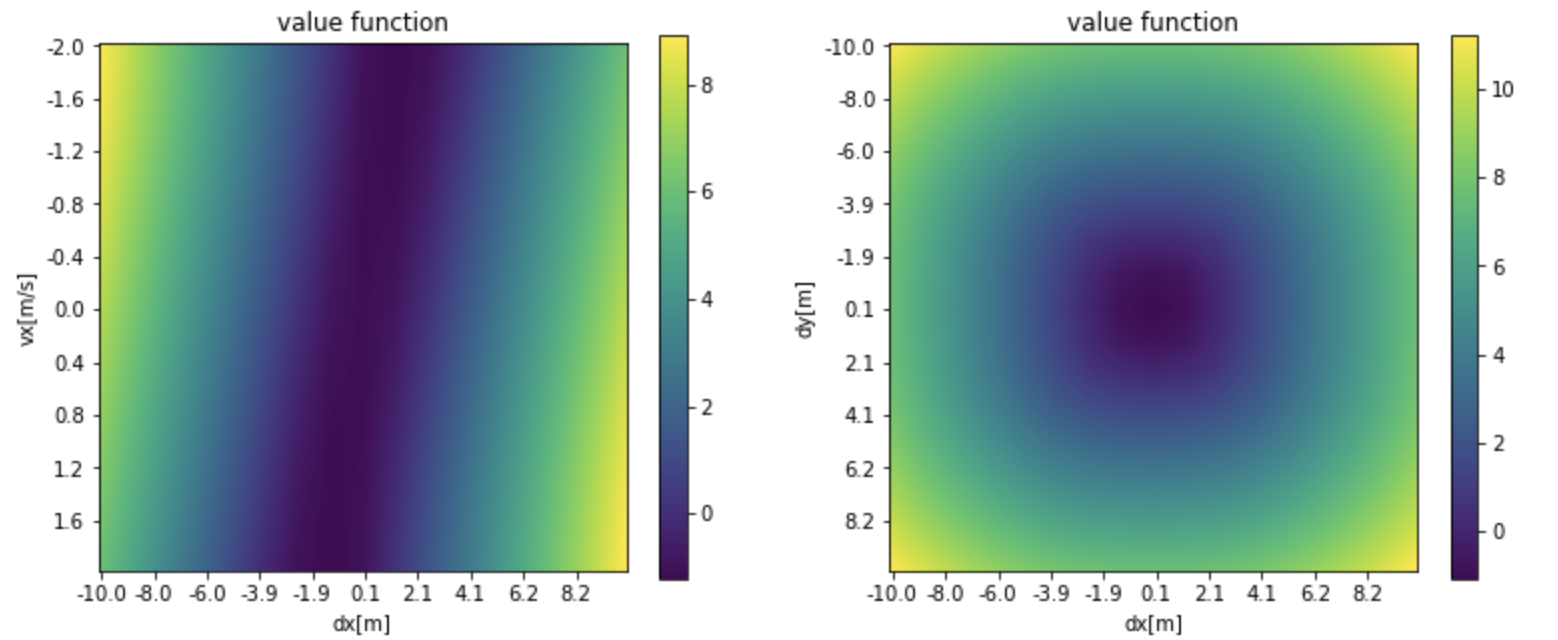
\includegraphics[width=\imgwidth]{images/hj_value_function.png}
\caption{2D slices of 4D \ac{HJR} value function: Position and velocity for one-dimensional case ($y = v_y = 0$, left) and two-dimensional static case ($v_x = v_y = 0$, right)}
\label{img:hj_value_function}
\end{center}
\end{figure}

\paragraph{Value Function approximation}
Due to the curse of dimensionality the value function cannot be determined with a resolution smaller than $0.5 m$ or $0.5 m/s$, with a feasible amount of pre-computation as well as size of the buffered value function grid and its gradients  on the RAM online \cite{Pavone2020}. There have been several methods for  approximating the value function in post-computation, such as \cite{Zhong2013} comparing the approximate performance of several regression classes such as nearest neighbor or locally weighted projection regression (LMDP) or \cite{Kuper2018} about verifiable safety-critical deep networks. It turns out that using nearest neighbor already lowers the control cost and improves stabilization capability of the value function based MPC control system for diverse (simple) experimental setups such as inverted pendulum, which holds even for time horizons $> 1.5s$. These results motivated comparing several interpolation methods for approximating the value function locally.

\begin{figure}[!ht]
\begin{center}
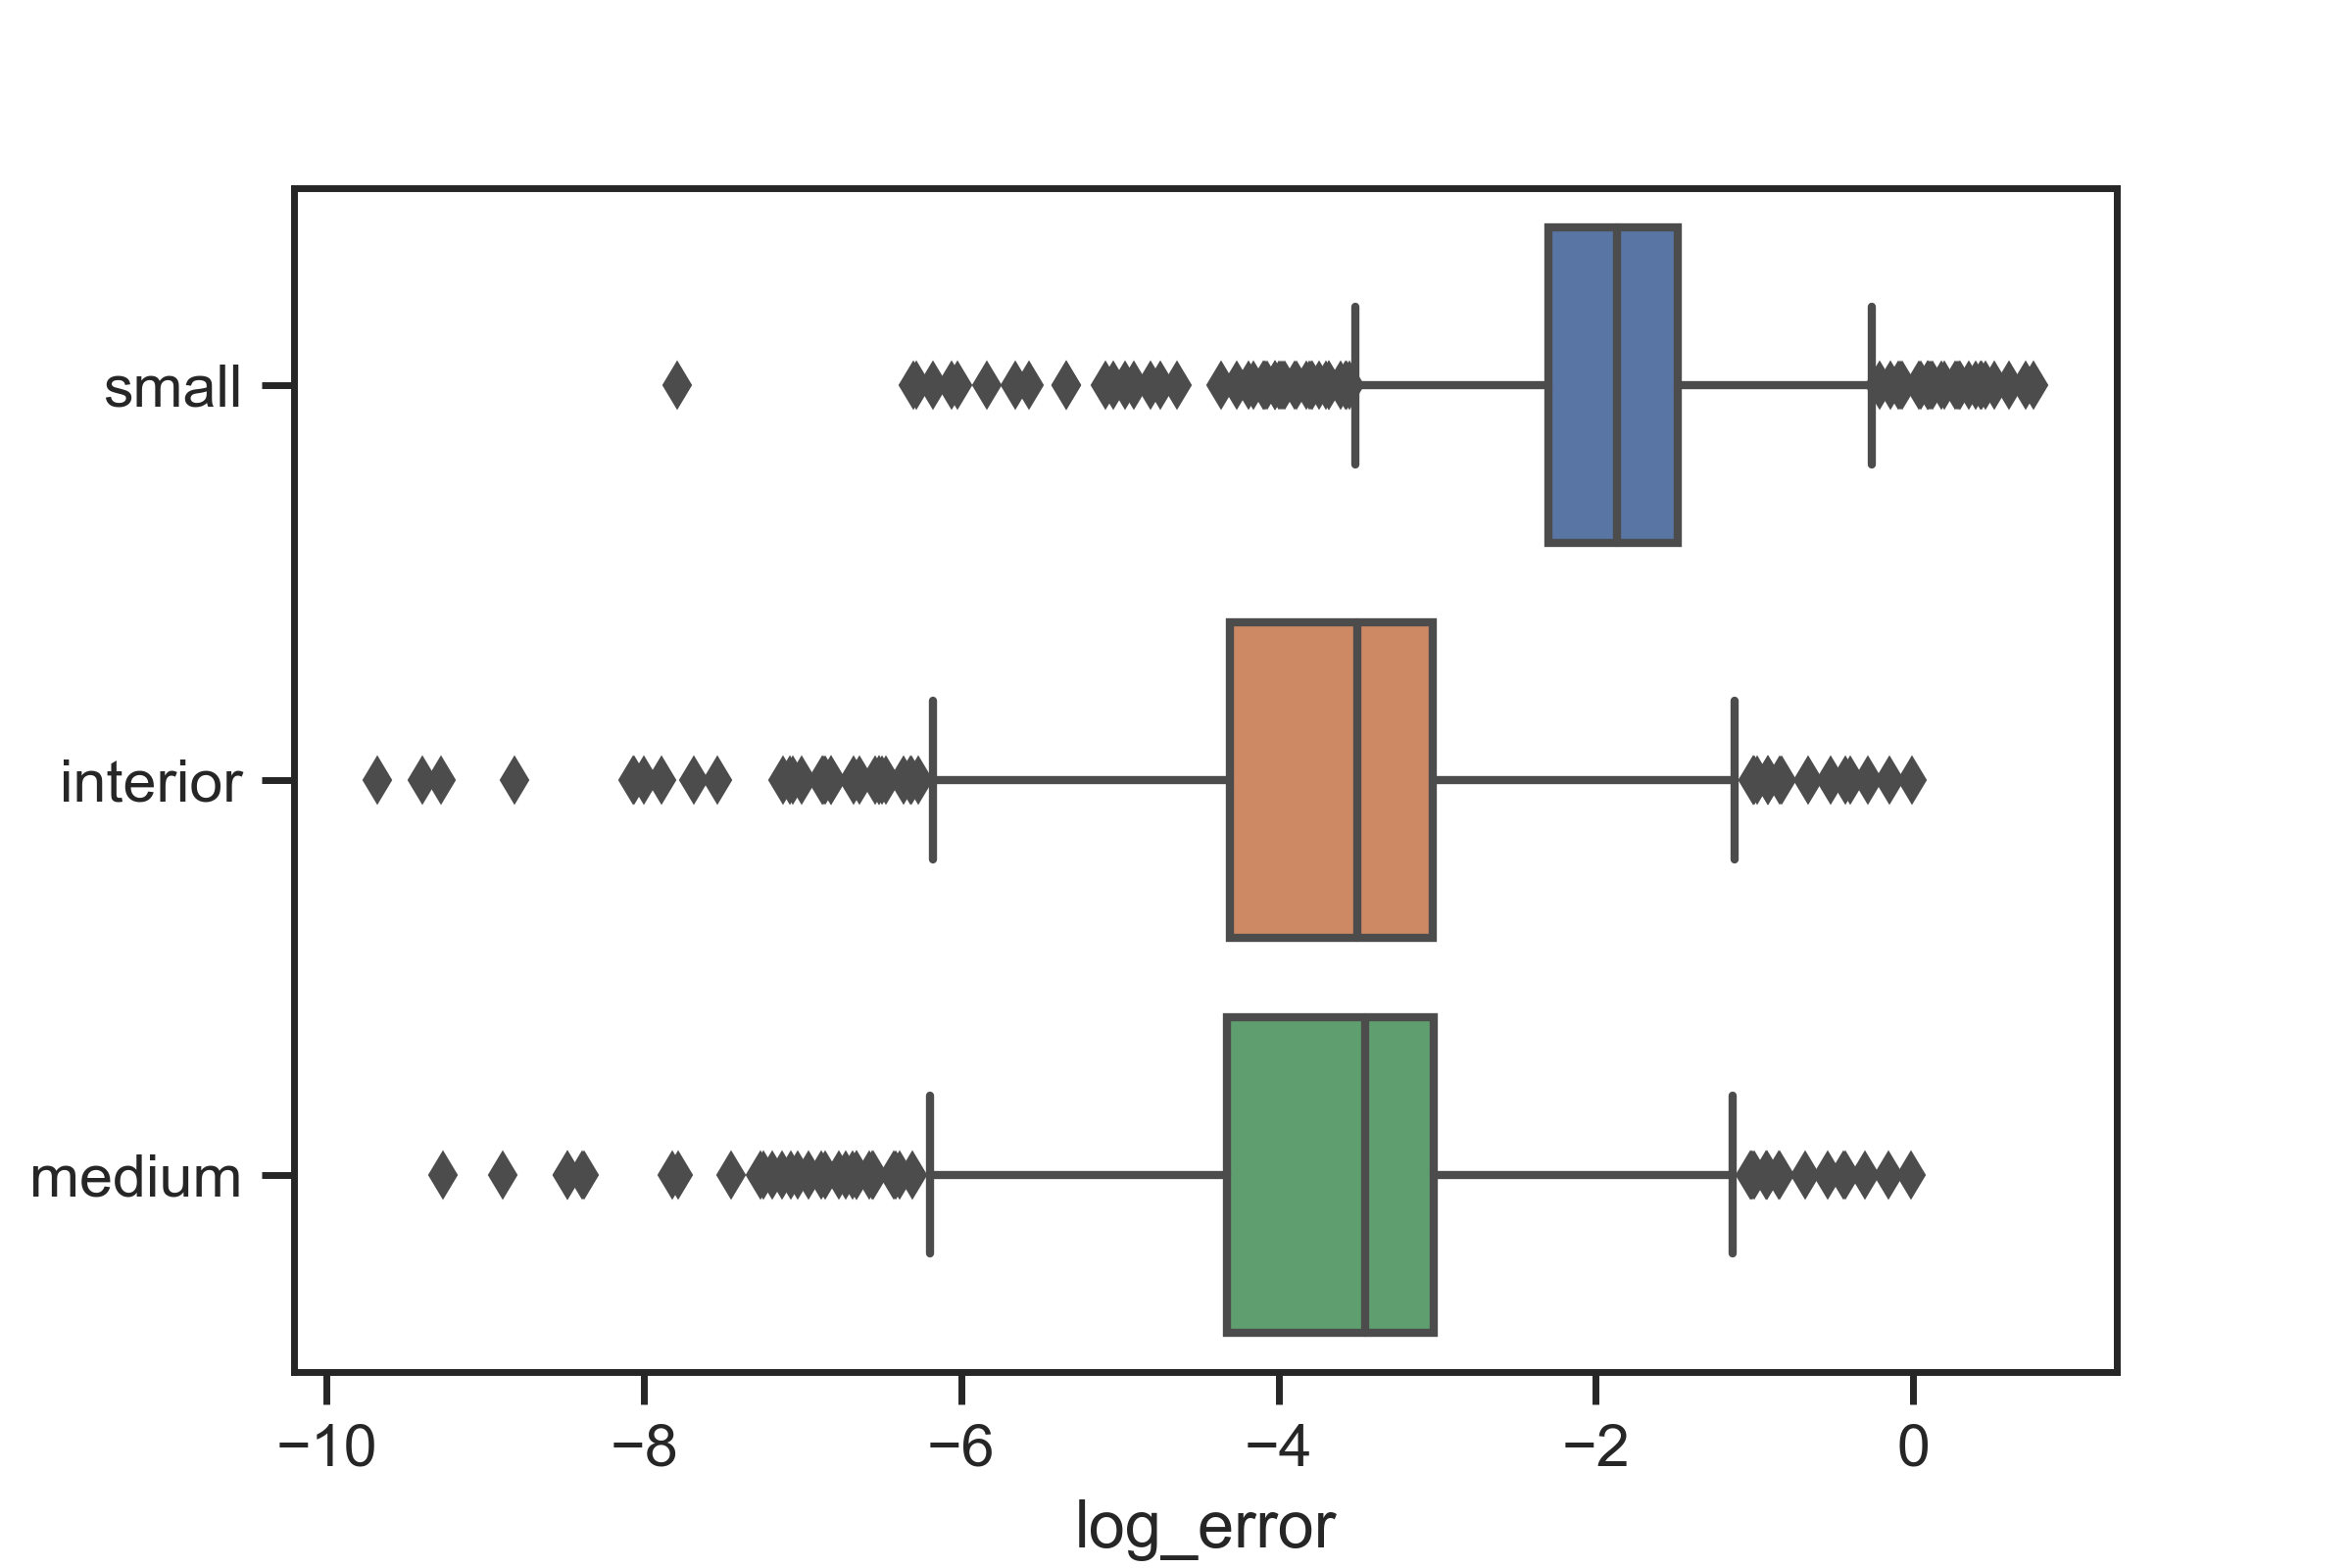
\includegraphics[width=0.45\textwidth]{images/hj_bar_linear.png}
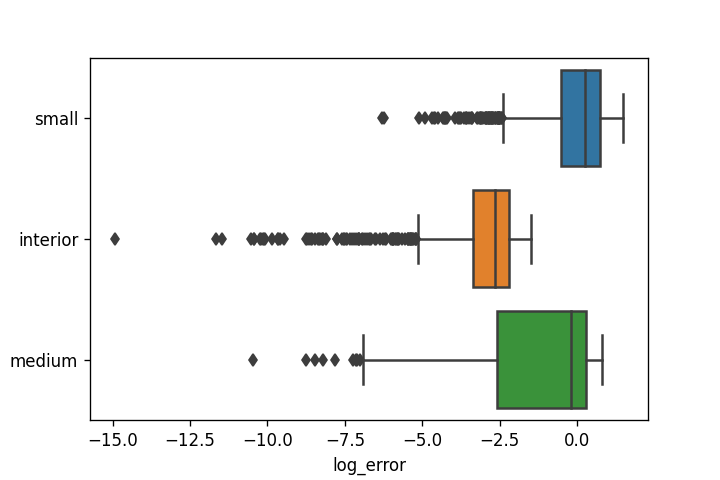
\includegraphics[width=0.45\textwidth]{images/hj_bar_nearest.png}
\caption{Logarithmic value function approximation error using linear (left) and nearest neighbor (right) interpolation methods based on various pre-computed grid sizes (small < interior < medium)}
\label{img:hj_approx_bar}
\end{center}
\end{figure}

\begin{figure}[!ht]
\begin{center}
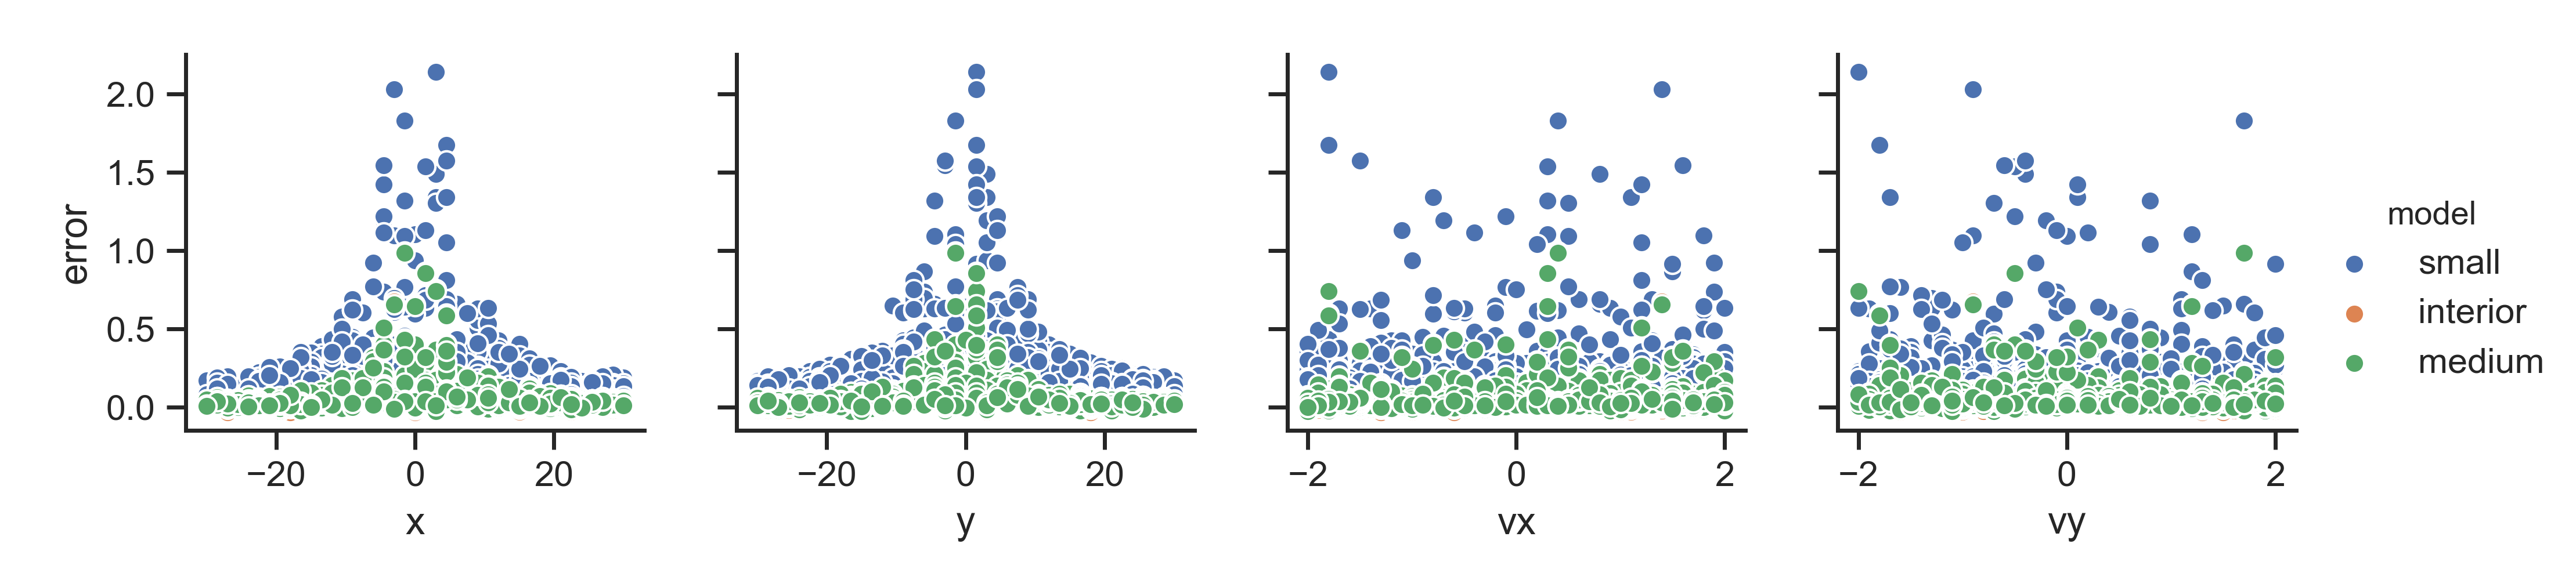
\includegraphics[width=\imgwidth]{images/hj_hist_linear.png}
\caption{Absolute error distribution over joint system state axes using linear interpolation based on various pre-computed grid sizes (small < interior < medium)}
\label{img:hj_approx_hist}
\end{center}
\end{figure}

Figure \ref{img:hj_approx_bar} shows the logarithmic approximation error for several pre-computed grid sizes and using linear (as in \cite{Leung2020}) and nearest neighbor interpolation methods. LWPR (not shown here) has been tested as well but turned out to be infeasible for a large amount of grid points.\footnote{For more information about the implementation of the LWPR value function approximation see \href{https://github.com/simon-schaefer/HJReachibility}{HJ-Reachability Toolbox} on GitHub.} For computing the error metric the value function has been computed on a dense grid exactly, and point-wise compared with the grid interpolated approximations. While linear interpolation widely outperforms nearest neighbor, as expected, the absolute error is very small. As displayed in Figure \ref{img:hj_approx_hist} the interpolation error is not uniform over all joint state axes, but larger for positional axes (which likely is due to the larger amount of non-linearity in position compared to velocity directions, compare Figure \ref{img:hj_value_function}). Therefore, the number of grid points have not been equally distributed over the axes, but biased to the positional axes (interior), while keeping the overall size of the grid constant. 

\paragraph{\ac{HJR} safety constraint} 
\cite{Leung2020} presents a safety-constraint, based on the resulting value function's gradient, by defining the set of safety-preserving robot control actions as:

\begin{equation}
\uset_{HJR} (\xrel) = \{ \u: \min_{\boldsymbol{d}} \nabla V (\xrel)^T \frel(\x, \boldsymbol{d}) \geq 0 \, | \, \u \in \uset \}
\end{equation}

Since the value function $V$ and its gradient $\nabla V$ are computed offline, the constraint is highly efficient to employ online. As the value function has been computed as backward reachable tube, when starting in a safe set $V > 0$ safety is guaranteed for feasible control actions, over the whole time-horizon $T_{HRJ}$, the value function was computed on. Especially, the constraint only depends on the current state, not on future states. Especially the last property make an \ac{HJR}-based constraint very well-suited for project \project. As previously stated evaluating as well as in particular backward passing through the prediction model is the optimization's computational bottleneck. An \ac{HJR}-based safety constraint as described above is however independent from the prediction model. 
\newline
In opposite to \cite{Leung2020} the value function for the joint robot-pedestrian system is negative almost everywhere (comp. Equation \ref{eq:hj_value_negative}), so that a safety-preserving constraint would be infeasible not matter which action is chosen. Therefore the value function itself is bounded, not pre-serving safety but guarantee to stay safe ($\Vrel \leq 0$).

\begin{align}
g_{HJR}(\x, \xped[], \u) &= \min_{\dxped[]} \Vrel(\xrel + \frel(\x, \xped[], \u, \dxped[]) \dt) \\
\uset_{HJR} (\xrel) &= \{ \u: g_{HJR}(\x, \xped[], \u) \geq \epsilon  \, | \, \u \in \uset \} 
\label{eq:hj_constraint}
\end{align}

To compute \ref{eq:hj_constraint} the value function for all possible pedestrian actions $\dxped[k]$ is determined, conditioned on the current relative state and the chosen robot's control action $\u$. The minimal value with respect to $\dxped[k]$, which reflects the value function in case of the worst-case scenario, given the robot's action, is constrained to be greater or equal zero. If $\u$ in $\uset_{HJR}$ then the robot is guaranteed to be safe from getting close to the pedestrian $k$ within the \ac{HJR}-time-horizon $T_{HJR} = 1s$. Additionally, the buffer $\epsilon > 0$ takes account for interpolation errors. 
\newline
In general it might occur that the relative state itself is infeasible, i.e. has a value term smaller than zero. Due to the inequality \ref{eq:hj_value_negative} there is no control action, that can be chosen by the robot, to reach a positive value. To avoid problem infeasibility, the constraint is appended by a slack variable $\eta \leq 0$, which is strongly weighted in the objective function. 

\begin{equation}
\uset_{HJR} (\xrel) = \{ \u: g_{HJR}(\x, \xped[], \u) + \eta \geq \epsilon  \, | \, \u \in \uset \}
\end{equation}

As the value function's gradient with respect to the relative state $\nabla \Vrel$ has been pre-computed, to determining the Jacobian of \ref{eq:hj_constraint} with respect to the robot's inputs, the chain rule is applied. Since the constraint only depends on the current joint state, as well as the planned initial control action of the robot, using \ref{eq:hj_dynamics} we have:

\begin{align}
\pd{g_{HJR}(\x, \xped[], \u)}{\u} &= \pd{\Vrel(\cdot}{\xrel + \frel(\cdot) \dt)} \pd{\xrel + \frel(\cdot) \dt)}{\u} \\ 
&= \nabla \Vrel^T(\cdot) \, \pd{\xrel + \frel(\cdot) \dt)}{\u} \\
&= \nabla \Vrel^T(\cdot) \, \left( \pd{\xrel}{\u} + \pd{\frel(\cdot) \dt}{\u} \right) \\ 
&= \nabla \Vrel^T(\cdot) \, \begin{bmatrix} 
\pd{\frel(\cdot) \dt}{\u_1} & 0 & 0 & \hdots \\ 
0 & 0 & 0 & \hdots \\ 
\vdots & \vdots & \vdots & \ddots \\ 
\end{bmatrix}
\end{align}

\paragraph{\ac{HJR} multi-agent coupling}
In reality, the a one-pedestrian scenario as depicted in Figure \ref{img:hj_game} rarely occurs, real scenarios are dynamic, not static, and involve the interactions between the robot and multiple agents, scenarios such the one indicated in Figure \ref{img:hj_game_multiagent}. Regarding Problem \ref{eq:hjr_problem} multiple agents pose a massive issue, since a joint state taking into account all the robot-pedestrian interactions would be much larger than four-dimensional, while even for simple dynamics a five- to six-dimensional state is the limit of computing the value function with a feasible amount of computational effort.
\newline
This problem can be solved by decomposing the joint system into sub-systems, solve \ref{eq:hjr_problem} for each of them individually and then intersect the back-projected sub-system solutions. \cite{Chen2016a} proves this method to result in an accurate representation of the full-system value function $\Vrel$, if the sub-systems are loosely coupled.

\begin{figure}[!ht]
\begin{center}
\begin{tikzpicture}

    \node[inner sep=0pt] (ped1) at (5,1)
    {
\includegraphics[width=.03\textwidth]{images/walking.png}};
    \fill[orange, opacity=0.3] (ped1) circle (1);
    \draw[dashed, ->] (ped1) to (4, 0);
    
    \node[inner sep=0pt] (ped2) at (-3,-1)
    {
\includegraphics[width=.03\textwidth]{images/walking.png}};
    \fill[orange, opacity=0.3] (ped2) circle (1);
    \draw[dashed, ->] (ped2) to (-1, 0);
    
    \node[inner sep=0pt] (ped3) at (0,2)
    {
\includegraphics[width=.03\textwidth]{images/walking.png}};
    \fill[orange, opacity=0.3] (ped3) circle (1);
    \draw[dashed, ->] (ped3) to (-1, 1);
    
    \node[inner sep=0pt] (ped4) at (2,-1)
    {
\includegraphics[width=.03\textwidth]{images/walking.png}};
    \fill[orange, opacity=0.3] (ped4) circle (1);
    \draw[dashed, ->] (ped4) to (1, -1);
    
    \node[inner sep=0pt] (robot) at (-0.5,0)
    {
\includegraphics[width=.04\textwidth]{images/robot.png}};
    
    \draw [thick] (robot) to[out=0, in=180] (5,3) to[out=0, in=180] node[above, sloped] {$\Vrel \geq 0$ ??} (10, 1);  
    
\end{tikzpicture}
\end{center}
\caption{Avoid set for static ($\dxped[]_t = 0$), single pedestrian scenario}
\label{img:hj_game_multiagent}
\end{figure}

Therefore we define the full system $z$ with uniformly continuous and for fixed control input $u$ bounded and Lipschitz continuous dynamics $f_{joint}: \mathcal{Z} \times \mathcal{U} \rightarrow \mathcal{Z}$. The system dynamics are generally described by an \ac{ODE} with solution with unique (!) solution trajectory $z^{\star} = \zeta(s; z, t, u)$, if $u$ is a measurable function (see \cite{Chen2016a}\cite{Varaiya1967}). Furthermore, the backward reachable set $\mathcal{V}(t)$ is defined as the set of states $z$ from which the system can arrive in an unsafe set $\mathcal{L}$ within time $t$. The subsystems $[1, \hdots, N_w]$ are described the projections of the full state $z$ onto the the sub-system state space $\mathcal{W}^i$, so that

\begin{align}
proj_{W^i}(z) &= w^i & \forall i \in [1, \hdots, N_s] \\
proj^{-1}(w^i) &= \{z \in \mathcal{Z}: proj_{W^i}(z) = w^i \} & \forall i \in [1, \hdots, N_w]
\label{eq:hj_projection}
\end{align}

Thereby a sub-system is any sub-set of the full joint state formulation, e.g. if $z = (y^1, y^2, y^3) \in \mathbb{R}^{n_z}$ then sub-systems might the pairs $w_1 = (y^1, y^2) \in \mathbb{R}^{n_1 + n_2}$ and $w_2 = (y^1, y^3) \in \mathbb{R}^{n_1 + n_3}$ with $n_1 + n_2 + n_3 = n_z$. These sub-systems are called self-contained if its dynamics solely depend on its states, not (explicitly) on the evolution of other sub-systems. Thereby note that sub-systems might still be coupled by a shared variable, as $y_1$ in the previous example.
\newline
In the following it shall be shown that the generalization of the system described in \ref{eq:hj_dynamics}, compromising a robot and multiple pedestrians can be decomposed into $M$ self-contained sub-systems where $M$ is the number of pedestrians in the full joint system: \\

\begin{corollary}
The full robot and $M$ pedestrians joint system dynamics can be written as 

\begin{equation}
\frel(\x, \xped[1], \xped[2], \hdots, \xped[M]) = 
\begin{bmatrix} 
\dx - \dxped[1] \\ 
\dx - \dxped[2] \\ 
\hdots \\
\dx - \dxped[M] \\ 
\u
\end{bmatrix}
\label{eq:hj_dynamics_full}
\end{equation}

The full coupled system $\mathcal{Z}_{rel} = (\x, \xped[1], \hdots, \xped[M])$ can be decomposed into sub-systems $\mathcal{W}_{rel}^i = (\x, \xped[i])$, which are self-contained. 
\label{co:hj_sub_systems}
\end{corollary}

\begin{proof}
Each sub-system $\mathcal{W}_{rel}^i$ follows the dynamics of a single pedestrian system as depicted above by Equations \ref{eq:hj_dynamics} and \ref{eq:hj_u_opt}. While in general the pedestrians might affect each other, as so by the internal structure of the prediction model $\distmodel[]$, this does not hold for the worst-case action that they are assumed to take. As shown for the single pedestrian scenario in Equation \ref{eq:hj_u_opt} the optimal disturbance regarding Problem \ref{eq:hjr_problem} is given by the maximal, or minimal, value of the pedestrian's velocity, depending on the sign of the value functions gradient. In particular, this policy and the speed limits are shared over all pedestrians. As a consequence the choice of the optimally disturbing action does not depend on the other pedestrians, the sub-systems are therefore only coupled by the robot's state and controls, while their evolvement does not depend on each other; and each are well-defined without the existence of the other. As a result, the sub-systems $\mathcal{W}_{rel}^i$ are self-contained.
\end{proof}

Given $N$ coupled systems, the intersection of the unsafe sets of each sub-system $\mathcal{L}_{\mathcal{w}_i}$, back-projected in the full joint state $z$ results in the full system's unsafe set $\mathcal{L}$. This is easy to see by plugging in $\mathcal{L}$ into \ref{eq:hj_projection}, yielding a superset of the actual sub-system's unsafe set. \cite{Chen2016a} proves that the same equality holds for the backward-reachable set, i.e. 

\begin{equation}
\Vrel(t) = proj^{-1}(\Vrel_{w_1}(t)) \cap proj^{-1}(\Vrel_{w_2}(t)) \cap \hdots \cap proj^{-1}(\Vrel_{w_M}(t))
\end{equation}

By implication, ssing \ref{co:hj_sub_systems} the full joint system's backward-reachable set can be expressed as the intersection of the back-projected sets of each subsystem. As the sub-systems are equal in terms of their dynamics, the sub-system's value function has to only be solved once, and evaluated and combined online.
